\section{Final Results}
As discussed in Section~\ref{sec:Optim}, the observed data were found to be consistent with the expected background.
Therefore, limits are placed on the production rate of various models of new physics. The statistical method used to determine the limits is discussed in
Section~\ref{sec:stats}. Figure~\ref{fig:MuExclusion}
shows the cross-section limit at 95\% confidence level (CL) for all considered models in the \muononly\ and \tktof\ analyses.
Figure~\ref{fig:TkExclusion} shows the same for the \tkonly\ and \multi\ analyses.

\begin{figure}
\centering
  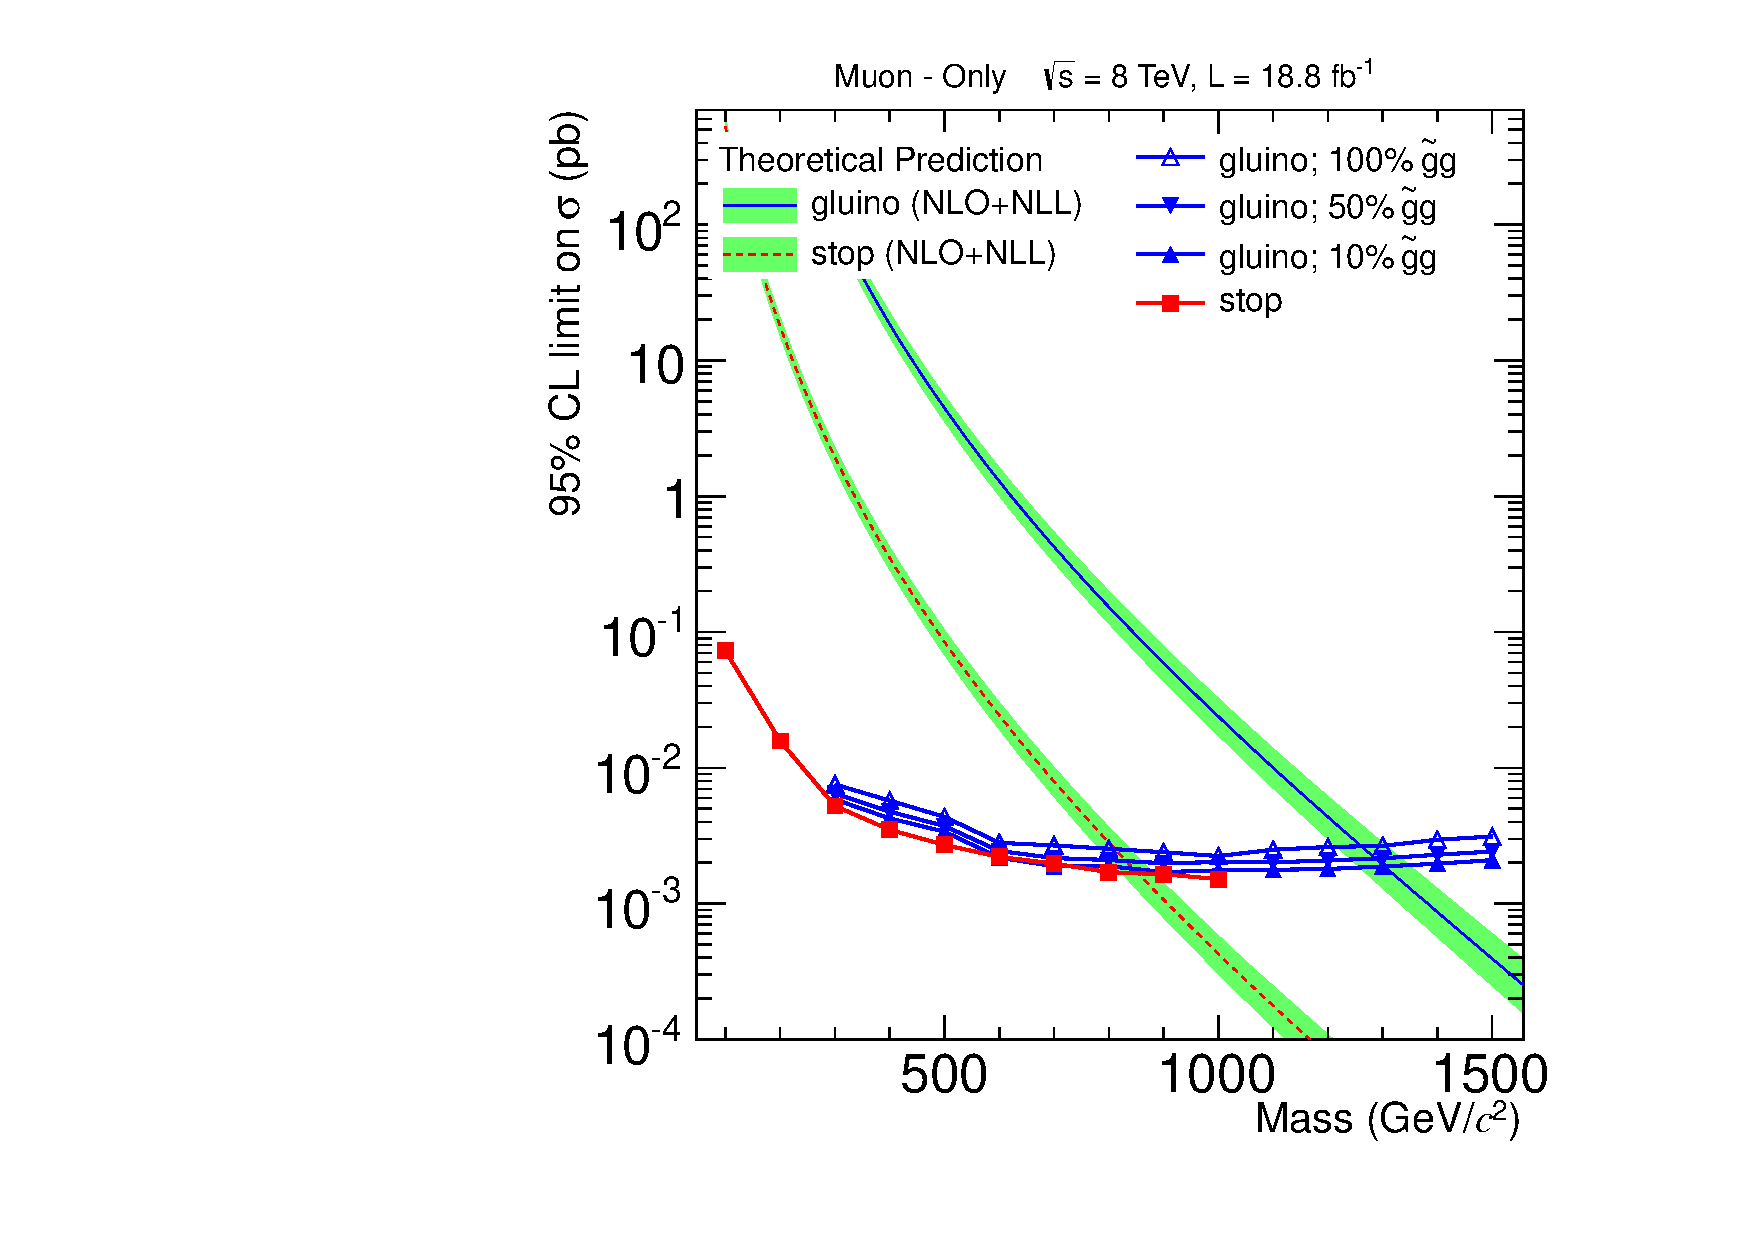
\includegraphics[clip=false, trim=0.0cm 0cm 0.0cm 0cm, width=0.48\textwidth]{figures/muonly/MOExclusionLog} \\
  \includegraphics[clip=false, trim=0.0cm 0cm 0.0cm 0cm, width=0.48\textwidth]{figures/tkmu/MuHadExclusionLog}
  \includegraphics[clip=false, trim=0.0cm 0cm 0.0cm 0cm, width=0.48\textwidth]{figures/tkmu/MuLepExclusionLog} \\
\caption[Cross-section limits obtained from 8~TeV data for all considered models in the \muononly\ and \tktof\ analyses]
{Cross-section limits obtained from 8~TeV data for all considered models in the \muononly\ (top) and \tktof\ (bottom) analyses.
The bottom left plot shows the limits for the \tktof\ analysis for hadron-like HSCP while the bottom right plot shows the limits for lepton-like HSCP.
}
    \label{fig:MuExclusion}
\end{figure}

\begin{figure}
\centering
  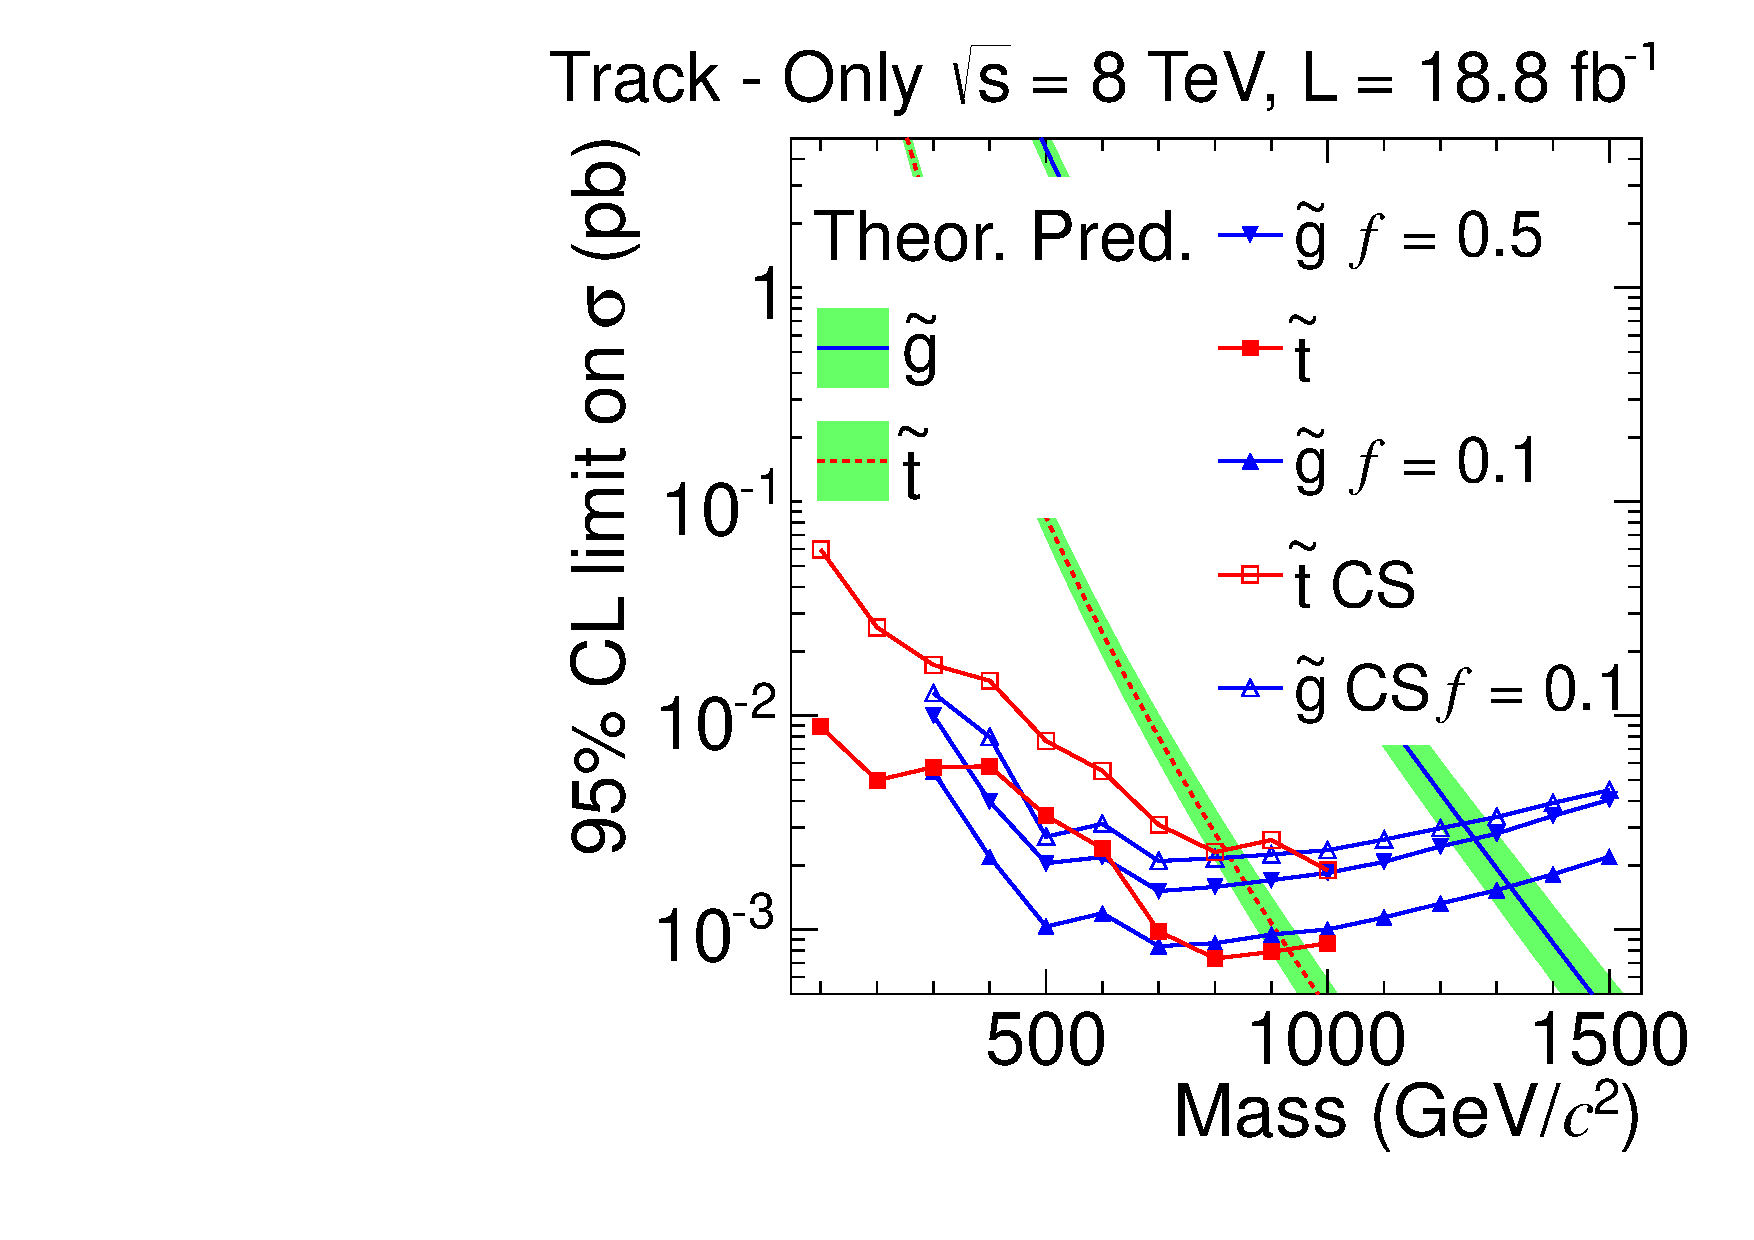
\includegraphics[clip=false, trim=0.0cm 0cm 0.0cm 0cm, width=0.48\textwidth]{figures/tkonly/TkExclusionLog} \\
  \includegraphics[clip=false, trim=0.0cm 0cm 0.0cm 0cm, width=0.48\textwidth]{figures/multi/HQLowExclusionLog}
  \includegraphics[clip=false, trim=0.0cm 0cm 0.0cm 0cm, width=0.48\textwidth]{figures/multi/HQHighExclusionLog}
\caption[Cross-section limits obtained from 8~TeV data for all considered models in the \tkonly\ and \multi\ analyses]
{Cross-section limits obtained from 8~TeV data for all considered models in the \tkonly\ (top) and \multi\ analyses.
The bottom left plot shows the limits for the \multi\ analysis for charges $<= 4e$ while the bottom right plot shows the limits for charges $> 4e$.
}
    \label{fig:TkExclusion}
\end{figure}

The CMS results for all the analyses except for \muononly\ combine the 8~TeV data collected in 2012 with 7~TeV data collected in 2011.
The combined result places limits on
the relative signal strength, $\sigma/\sigma_{th}$. The 7~TeV results are simply added here without further description.
The limits on the relative cross-section
for the \muononly\ and \tktof\ analyses is shown in Figure~\ref{fig:MuRelExclusion}. For the \muononly\ analysis the limit on signal strength uses only 8~TeV data.
The limits on the relative cross-section for the \tkonly\ and \multi\ analyses is shown in Figure~\ref{fig:TkRelExclusion}.

\begin{figure}
\centering
  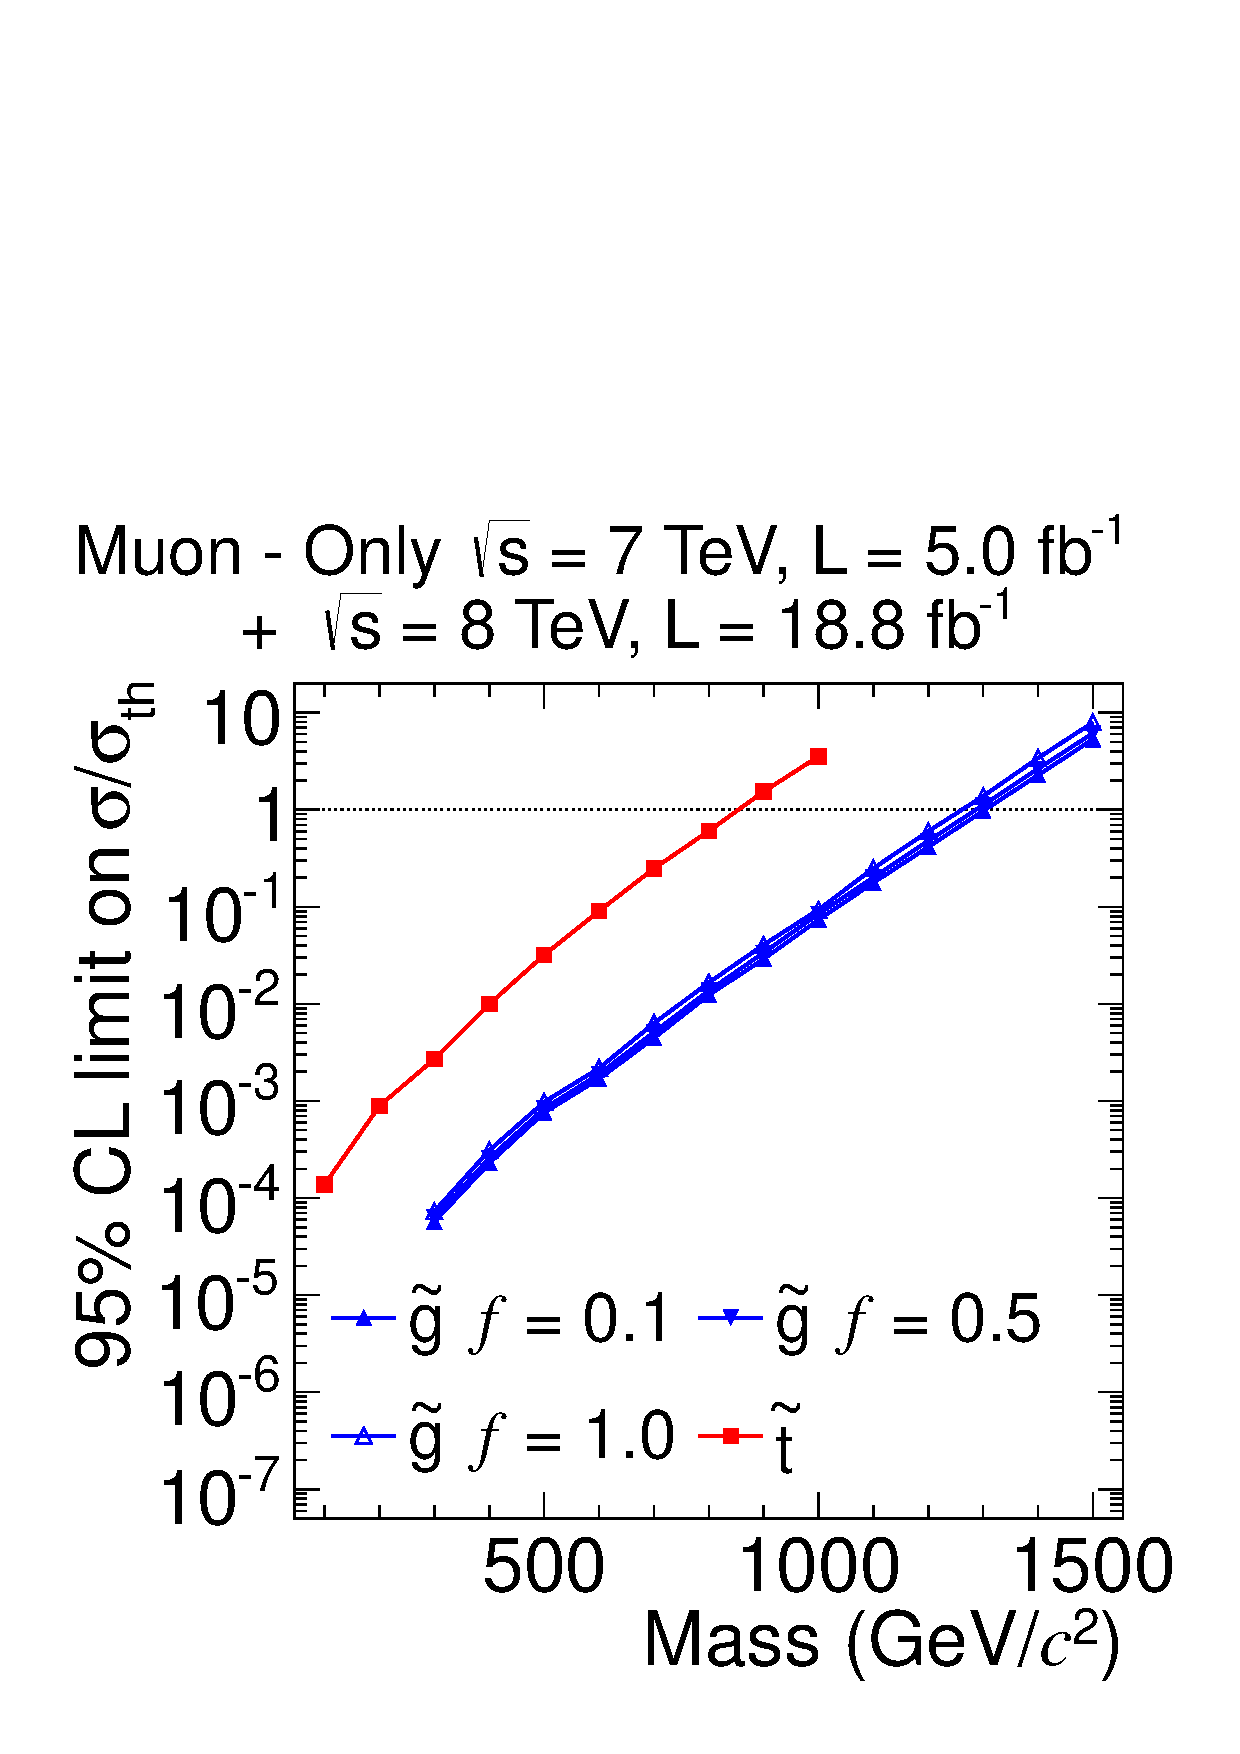
\includegraphics[clip=false, trim=0.0cm 0cm 0.0cm 0cm, width=0.48\textwidth]{figures/muonly/MOExclusionRelLog} \\
  \includegraphics[clip=false, trim=0.0cm 0cm 0.0cm 0cm, width=0.48\textwidth]{figures/tkmu/MuHadExclusionRelLog}
  \includegraphics[clip=false, trim=0.0cm 0cm 0.0cm 0cm, width=0.48\textwidth]{figures/tkmu/MuLepExclusionRelLog} \\
\caption[Limits on the relative signal strength, $\sigma/\sigma_{th}$, set by the \muononly\ and \tktof\ analyses]
{Limits on the relative signal strength, $\sigma/\sigma_{th}$,  set by the \muononly\ (top) and \tktof\ (bottom) analyses.
The bottom left plot shows the limits for the \tktof\ analysis for hadron-like HSCP while the bottom right plot shows the limits for lepton-like HSCP.
}
    \label{fig:MuRelExclusion}
\end{figure}

\begin{figure}
\centering
  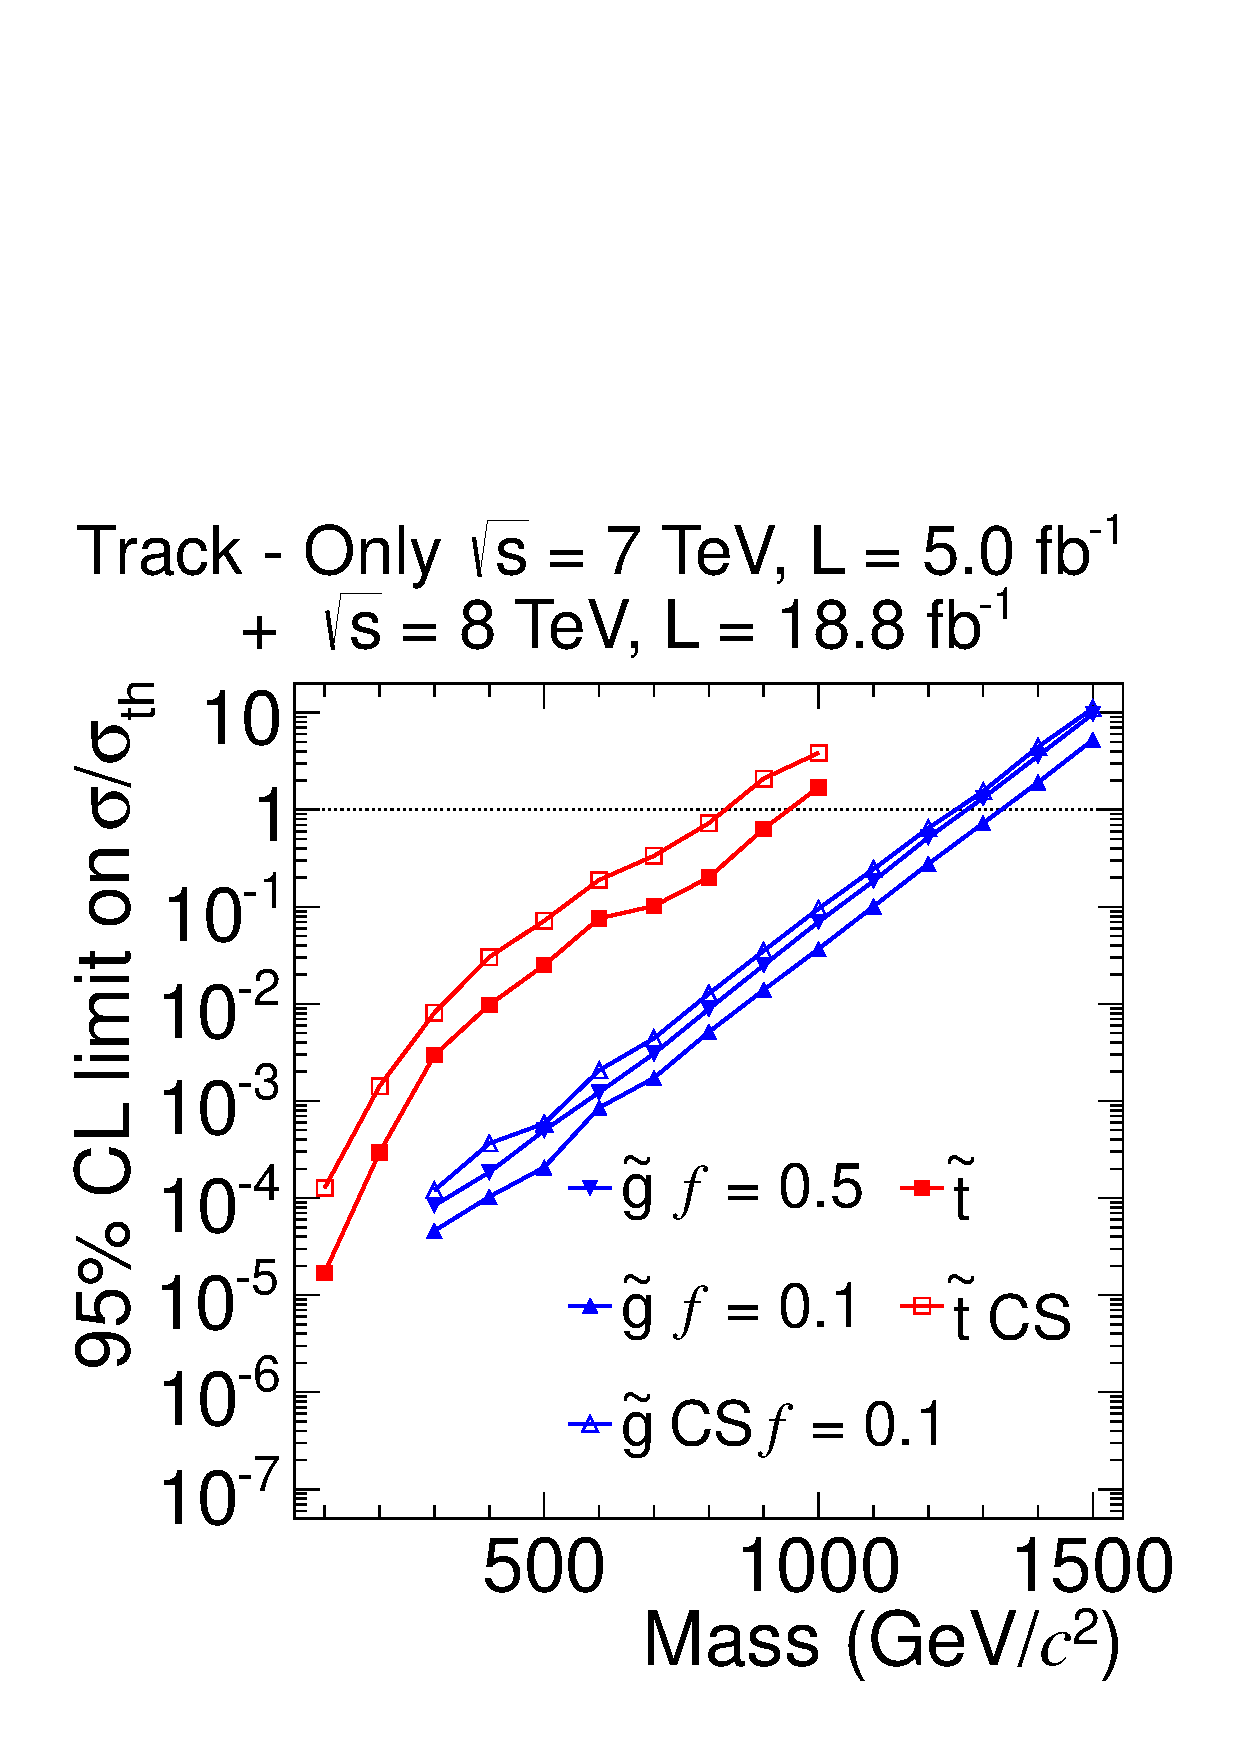
\includegraphics[clip=false, trim=0.0cm 0cm 0.0cm 0cm, width=0.48\textwidth]{figures/tkonly/TkExclusionRelLog} \\
  \includegraphics[clip=false, trim=0.0cm 0cm 0.0cm 0cm, width=0.48\textwidth]{figures/multi/HQLowExclusionRelLog}
  \includegraphics[clip=false, trim=0.0cm 0cm 0.0cm 0cm, width=0.48\textwidth]{figures/multi/HQHighExclusionRelLog}
\caption[Limits on the relative signal strength, $\sigma/\sigma_{th}$, set by the \tkonly\ and \multi\ analyses]
{Limits on the relative signal strength, $\sigma/\sigma_{th}$,  set by the \tkonly\ (top) and \multi\ analyses.
The bottom left plot shows the limits for the \multi\ analysis for charges $<= 4e$ while the bottom right plot shows the limits for charges $> 4e$.
}
    \label{fig:TkRelExclusion}
\end{figure}

Table~\ref{tab:SummaryMuOnly} has the observed and expected limits for all the signal points in the \muononly\ analysis as well as the signal efficiency. 
Table~\ref{tab:SummaryTkTOF} shows the same for the \tktof\ analysis. Tables~\ref{tab:SummaryTkOnly} and~\ref{tab:SummaryMulti} show the efficiency
and observed and expected limits for some of the signal points in the \tkonly\ and \multi\ analyses, respectively.

\begin{center}
\begin{longtable}{|c|ccc|cc|}
\caption[Summary table of results for all the considered signal points for the \muononly\ analysis.]
{Summary table of results for all the considered signal points for the \muononly\ analysis.
The signal efficiency and observed and expected limits on the cross section (in $pb$) at $\sqrt{s} = 8$~TeV are presented.
Also the observed and expected limits on the signal strength at $\sqrt{s} = 8$~TeV.
  \label{tab:SummaryMuOnly}}  \\
\hline
Mass  & \multicolumn{3}{c|}{$\sigma (pb)$} & \multicolumn{2}{c|}{$\mu = \sigma/\sigma_{TH}$} \\
(GeV$/c^2$) & \multicolumn{3}{c|}{$\sqrt{s}=8TeV$} & \multicolumn{2}{c|}{$\sqrt{s} = 8$~TeV} \\
      & Eff. & Obs. & Exp. & Obs. & Exp. \\
\hline
\endfirsthead
\multicolumn{6}{c}%
{\tablename\ \thetable\ -- \textit{Continued from previous page}} \\
\hline
Mass  & \multicolumn{3}{c|}{$\sigma$~(pb)} & \multicolumn{2}{c|}{$\mu = \sigma/\sigma_{TH}$} \\
(GeV$/c^2$) & \multicolumn{3}{c|}{$\sqrt{s}=8TeV$} & \multicolumn{2}{c|}{$\sqrt{s} = 8$~TeV} \\
      & Eff. & Obs. & Exp. & Obs. & Exp. \\
\hline
\endhead
\hline
\multicolumn{6}{r}{\textit{Continued on next page}} \\
\endfoot
\endlastfoot
 \multicolumn{6}{|c|}{Gluino 100\% $\tilde{g}g$ ~~~-~~~ \muononly\ analysis} \\ \hline
 300 & 0.050 & 0.0075 & 0.0070 & $      7.3 \times 10^{-5}$ & $      6.8 \times 10^{-5}$\\
 400 & 0.066 & 0.0057 & 0.0050 & $      3.1 \times 10^{-4}$ & $      2.7 \times 10^{-4}$\\
 500 & 0.086 & 0.0044 & 0.0037 & $      9.8 \times 10^{-4}$ & $      8.4 \times 10^{-4}$\\
 600 & 0.096 & 0.0028 & 0.0034 & 0.0022 & 0.0026\\
 700 & 0.10 & 0.0027 & 0.0032 & 0.0063 & 0.0075\\
 800 & 0.11 & 0.0025 & 0.0030 & 0.017 & 0.020\\
 900 & 0.11 & 0.0024 & 0.0029 & 0.041 & 0.049\\
1000 & 0.11 & 0.0022 & 0.0030 & 0.094 & 0.12\\
1100 & 0.11 & 0.0025 & 0.0030 & 0.25 & 0.30\\
1200 & 0.10 & 0.0026 & 0.0032 & 0.60 & 0.73\\
1300 & 0.10 & 0.0027 & 0.0032 & 1.4 & 1.7\\
1400 & 0.092 & 0.0030 & 0.0036 & 3.4 & 4.1\\
1500 & 0.087 & 0.0031 & 0.0037 & 7.9 & 9.5\\ \hline
 \multicolumn{6}{|c|}{Gluino 50\% $\tilde{g}g$ ~~~-~~~ \muononly\ analysis} \\ \hline
 300 & 0.058 & 0.0065 & 0.0060 & $      6.3 \times 10^{-5}$ & $      5.8 \times 10^{-5}$\\
 400 & 0.079 & 0.0048 & 0.0041 & $      2.6 \times 10^{-4}$ & $      2.2 \times 10^{-4}$\\
 500 & 0.10 & 0.0037 & 0.0032 & $      8.3 \times 10^{-4}$ & $      7.2 \times 10^{-4}$\\
 600 & 0.11 & 0.0024 & 0.0028 & 0.0019 & 0.0022\\
 700 & 0.12 & 0.0022 & 0.0026 & 0.0051 & 0.0062\\
 800 & 0.13 & 0.0021 & 0.0025 & 0.014 & 0.017\\
 900 & 0.14 & 0.0020 & 0.0024 & 0.034 & 0.041\\
1000 & 0.13 & 0.0020 & 0.0024 & 0.085 & 0.10\\
1100 & 0.13 & 0.0020 & 0.0024 & 0.20 & 0.24\\
1200 & 0.13 & 0.0021 & 0.0025 & 0.48 & 0.58\\
1300 & 0.12 & 0.0022 & 0.0026 & 1.1 & 1.4\\
1400 & 0.12 & 0.0023 & 0.0028 & 2.6 & 3.2\\
1500 & 0.11 & 0.0024 & 0.0030 & 6.2 & 7.5\\ \hline
 \multicolumn{6}{|c|}{Gluino 10\% $\tilde{g}g$ ~~~-~~~ \muononly\ analysis} \\ \hline
 300 & 0.064 & 0.0058 & 0.0054 & $      5.7 \times 10^{-5}$ & $      5.3 \times 10^{-5}$\\
 400 & 0.089 & 0.0042 & 0.0037 & $      2.3 \times 10^{-4}$ & $      2.0 \times 10^{-4}$\\
 500 & 0.11 & 0.0034 & 0.0029 & $      7.6 \times 10^{-4}$ & $      6.6 \times 10^{-4}$\\
 600 & 0.13 & 0.0022 & 0.0026 & 0.0017 & 0.0020\\
 700 & 0.14 & 0.0019 & 0.0023 & 0.0044 & 0.0055\\
 800 & 0.15 & 0.0019 & 0.0022 & 0.012 & 0.015\\
 900 & 0.15 & 0.0017 & 0.0021 & 0.029 & 0.036\\
1000 & 0.15 & 0.0018 & 0.0021 & 0.074 & 0.089\\
1100 & 0.15 & 0.0018 & 0.0021 & 0.18 & 0.21\\
1200 & 0.15 & 0.0018 & 0.0022 & 0.41 & 0.51\\
1300 & 0.14 & 0.0019 & 0.0023 & 0.97 & 1.2\\
1400 & 0.14 & 0.0020 & 0.0024 & 2.3 & 2.8\\
1500 & 0.13 & 0.0021 & 0.0026 & 5.3 & 6.5\\ \hline
 \multicolumn{6}{|c|}{Stop ~~~-~~~ \muononly\ analysis} \\ \hline
 100 & 0.0052 & 0.073 & 0.063 & $      1.4 \times 10^{-4}$ & $      1.2 \times 10^{-4}$\\
 200 & 0.024 & 0.016 & 0.014 & $      8.9 \times 10^{-4}$ & $      7.8 \times 10^{-4}$\\
 300 & 0.050 & 0.0052 & 0.0066 & 0.0027 & 0.0034\\
 400 & 0.078 & 0.0035 & 0.0042 & 0.010 & 0.012\\
 500 & 0.10 & 0.0027 & 0.0033 & 0.032 & 0.039\\
 600 & 0.12 & 0.0022 & 0.0027 & 0.090 & 0.11\\
 700 & 0.14 & 0.0020 & 0.0024 & 0.25 & 0.30\\
 800 & 0.15 & 0.0017 & 0.0021 & 0.60 & 0.75\\
 900 & 0.17 & 0.0016 & 0.0020 & 1.5 & 1.8\\
1000 & 0.18 & 0.0015 & 0.0019 & 3.5 & 4.4\\ \hline
\end{longtable}
\end{center}



\begin{center}
\begin{longtable}{|c|c|ccc|cc|}
\caption[Summary table of results for all the considered signal points for the \tktof\ analysis.]
{Summary table of results for all the considered signal points for the \tktof\ analysis.
  The signal efficiency and observed and expected limits on the cross section (in $pb$) at $\sqrt{s} = 8$~TeV.
Also the observed and expected limits on the signal strength at $\sqrt{s} =$ 7 and 8~TeV.
  \label{tab:SummaryTkTOF}}  \\
\hline
Mass  & Mass & \multicolumn{3}{c|}{$\sigma$~(pb)} & \multicolumn{2}{c|}{$\mu = \sigma/\sigma_{TH}$} \\
(GeV$/c^2$) & Req. & \multicolumn{3}{c|}{$\sqrt{s}=8TeV$} & \multicolumn{2}{c|}{$\sqrt{s} =$ 7 and 8~TeV} \\
      & (GeV$/c^2$) & Eff. & Obs. & Exp. & Obs. & Exp. \\
\hline
\endfirsthead
\multicolumn{7}{c}%
{\tablename\ \thetable\ -- \textit{Continued from previous page}} \\
\hline
Mass  & Mass & \multicolumn{3}{c|}{$\sigma$~(pb)} & \multicolumn{2}{c|}{$\mu = \sigma/\sigma_{TH}$} \\
(GeV$/c^2$) & Req. & \multicolumn{3}{c|}{$\sqrt{s}=8TeV$} & \multicolumn{2}{c|}{$\sqrt{s} =$ 7 and 8~TeV} \\
      & (GeV$/c^2$) & Eff. & Obs. & Exp. & Obs. & Exp. \\
\hline
\endhead
\hline
\multicolumn{7}{r}{\textit{Continued on next page}} \\
\endfoot
\endlastfoot
 \multicolumn{7}{|c|}{CD Stau ~~~-~~~ \tktof\ analysis} \\ \hline
 100 & $>20$   & 0.16 & 0.0062 & 0.0063 & 0.0023 & 0.0025\\
 126 & $>40$   & 0.25 & 0.0042 & 0.0042 & 0.0065 & 0.0074\\
 156 & $>70$   & 0.32 & 0.0024 & 0.0017 & 0.017 & 0.013\\
 200 & $>110$  & 0.41 & 0.0012 & $      7.7 \times 10^{-4}$ & 0.056 & 0.031\\
 247 & $>150$  & 0.50 & $      8.1 \times 10^{-4}$ & $      4.4 \times 10^{-4}$ & 0.15 & 0.068\\
 308 & $>190$  & 0.56 & $      2.8 \times 10^{-4}$ & $      2.9 \times 10^{-4}$ & 0.21 & 0.16\\
 370 & $>240$  & 0.60 & $      2.7 \times 10^{-4}$ & $      2.6 \times 10^{-4}$ & 0.40 & 0.38\\
 432 & $>290$  & 0.64 & $      2.5 \times 10^{-4}$ & $      2.3 \times 10^{-4}$ & 0.92 & 0.86\\
 494 & $>330$  & 0.66 & $      2.5 \times 10^{-4}$ & $      2.3 \times 10^{-4}$ & 1.9 & 1.9\\ \hline
 \multicolumn{7}{|c|}{DP ~~~-~~~ \tktof\ analysis} \\ \hline
 100 & $>20$   & 0.17 & 0.0056 & 0.0062 & 0.099 & 0.11\\
 126 & $>40$   & 0.24 & 0.0043 & 0.0044 & 0.16 & 0.18\\
 156 & $>60$   & 0.28 & 0.0027 & 0.0024 & 0.23 & 0.21\\
 200 & $>100$  & 0.34 & 0.0013 & 0.0010 & 0.42 & 0.26\\
 247 & $>140$  & 0.40 & $      9.9 \times 10^{-4}$ & $      5.8 \times 10^{-4}$ & 0.85 & 0.37\\
 308 & $>190$  & 0.46 & $      3.5 \times 10^{-4}$ & $      3.5 \times 10^{-4}$ & 0.66 & 0.62\\
 370 & $>240$  & 0.53 & $      3.0 \times 10^{-4}$ & $      2.9 \times 10^{-4}$ & 1.4 & 1.2\\
 432 & $>280$  & 0.57 & $      2.9 \times 10^{-4}$ & $      2.6 \times 10^{-4}$ & 2.5 & 2.4\\
 494 & $>330$  & 0.61 & $      2.6 \times 10^{-4}$ & $      2.5 \times 10^{-4}$ & 5.0 & 4.7\\ \hline
 \multicolumn{7}{|c|}{Gluino 50\% $\tilde{g}g$ ~~~-~~~ \tktof\ analysis} \\ \hline
 300 & $>110$  & 0.075 & 0.0044 & 0.0041 & $      5.0 \times 10^{-5}$ & $      3.1 \times 10^{-5}$\\
 400 & $>190$  & 0.085 & 0.0021 & 0.0020 & $      9.6 \times 10^{-5}$ & $      9.3 \times 10^{-5}$\\
 500 & $>260$  & 0.091 & 0.0021 & 0.0016 & $      2.8 \times 10^{-4}$ & $      3.1 \times 10^{-4}$\\
 600 & $>330$  & 0.092 & 0.0018 & 0.0016 & 0.0012 & 0.0011\\
 700 & $>400$  & 0.090 & 0.0018 & 0.0018 & 0.0037 & 0.0034\\
 800 & $>480$  & 0.083 & 0.0019 & 0.0019 & 0.011 & 0.010\\
 900 & $>530$  & 0.076 & 0.0021 & 0.0020 & 0.031 & 0.029\\
1000 & $>610$  & 0.068 & 0.0023 & 0.0023 & 0.085 & 0.082\\
1100 & $>660$  & 0.059 & 0.0028 & 0.0026 & 0.24 & 0.23\\
1200 & $>710$  & 0.047 & 0.0034 & 0.0032 & 0.69 & 0.66\\
1300 & $>750$  & 0.039 & 0.0041 & 0.0039 & 1.9 & 1.8\\
1400 & $>800$  & 0.030 & 0.0054 & 0.0051 & 5.7 & 5.3\\
1500 & $>830$  & 0.023 & 0.0069 & 0.0066 & 17. & 16.\\ \hline
 \multicolumn{7}{|c|}{Gluino 10\% $\tilde{g}g$ ~~~-~~~ \tktof\ analysis} \\ \hline
 300 & $>110$  & 0.14 & 0.0024 & 0.0022 & $      2.6 \times 10^{-5}$ & $      1.7 \times 10^{-5}$\\
 400 & $>190$  & 0.15 & 0.0011 & 0.0011 & $      5.6 \times 10^{-5}$ & $      5.1 \times 10^{-5}$\\
 500 & $>260$  & 0.16 & 0.0011 & $      8.7 \times 10^{-4}$ & $      1.6 \times 10^{-4}$ & $      1.8 \times 10^{-4}$\\
 600 & $>330$  & 0.17 & $      8.7 \times 10^{-4}$ & $      9.1 \times 10^{-4}$ & $      6.0 \times 10^{-4}$ & $      6.0 \times 10^{-4}$\\
 700 & $>410$  & 0.16 & $      9.6 \times 10^{-4}$ & 0.0010 & 0.0021 & 0.0017\\
 800 & $>480$  & 0.15 & 0.0011 & 0.0010 & 0.0058 & 0.0057\\
 900 & $>540$  & 0.14 & 0.0012 & 0.0011 & 0.017 & 0.016\\
1000 & $>610$  & 0.12 & 0.0013 & 0.0012 & 0.046 & 0.045\\
1100 & $>660$  & 0.11 & 0.0015 & 0.0014 & 0.13 & 0.12\\
1200 & $>710$  & 0.089 & 0.0018 & 0.0017 & 0.37 & 0.35\\
1300 & $>750$  & 0.072 & 0.0022 & 0.0021 & 1.0 & 0.99\\
1400 & $>800$  & 0.056 & 0.0029 & 0.0027 & 2.9 & 2.8\\
1500 & $>830$  & 0.043 & 0.0037 & 0.0035 & 8.6 & 8.1\\ \hline
 \multicolumn{7}{|c|}{Stop ~~~-~~~ \tktof\ analysis} \\ \hline
 100 & $>0$    & 0.057 & 0.019 & 0.019 & $      3.0 \times 10^{-5}$ & $      2.8 \times 10^{-5}$\\
 200 & $>0$    & 0.12 & 0.0088 & 0.0085 & $      4.0 \times 10^{-4}$ & $      2.6 \times 10^{-4}$\\
 300 & $>20$   & 0.15 & 0.0068 & 0.0069 & 0.0024 & 0.0019\\
 400 & $>80$   & 0.16 & 0.0039 & 0.0028 & 0.0072 & 0.0055\\
 500 & $>140$  & 0.17 & 0.0022 & 0.0013 & 0.019 & 0.013\\
 600 & $>210$  & 0.18 & $      8.8 \times 10^{-4}$ & $      9.1 \times 10^{-4}$ & 0.031 & 0.031\\
 700 & $>290$  & 0.17 & $      9.4 \times 10^{-4}$ & $      8.8 \times 10^{-4}$ & 0.099 & 0.094\\
 800 & $>370$  & 0.17 & $      9.7 \times 10^{-4}$ & $      9.1 \times 10^{-4}$ & 0.29 & 0.27\\
 900 & $>450$  & 0.15 & 0.0011 & 0.0010 & 0.84 & 0.79\\
1000 & $>530$  & 0.13 & 0.0012 & 0.0012 & 2.5 & 2.3\\ \hline
 \multicolumn{7}{|c|}{DY Q = 1e ~~~-~~~ \tktof\ analysis} \\ \hline
 100 & $>40$   & 0.15 & 0.0068 & 0.0069 & 0.011 & 0.012\\
 200 & $>120$  & 0.36 & 0.0013 & $      7.7 \times 10^{-4}$ & 0.040 & 0.019\\
 300 & $>190$  & 0.48 & $      3.3 \times 10^{-4}$ & $      3.4 \times 10^{-4}$ & 0.060 & 0.046\\
 400 & $>270$  & 0.53 & $      3.0 \times 10^{-4}$ & $      2.9 \times 10^{-4}$ & 0.15 & 0.14\\
 500 & $>340$  & 0.56 & $      2.9 \times 10^{-4}$ & $      2.8 \times 10^{-4}$ & 0.44 & 0.41\\
 600 & $>400$  & 0.56 & $      2.9 \times 10^{-4}$ & $      2.8 \times 10^{-4}$ & 1.2 & 1.1\\
 700 & $>470$  & 0.55 & $      3.0 \times 10^{-4}$ & $      2.8 \times 10^{-4}$ & 3.1 & 3.0\\
 800 & $>530$  & 0.52 & $      3.1 \times 10^{-4}$ & $      3.0 \times 10^{-4}$ & 8.1 & 7.5\\
 900 & $>590$  & 0.49 & $      3.3 \times 10^{-4}$ & $      3.2 \times 10^{-4}$ & 20. & 19.\\
1000 & $>650$  & 0.45 & $      3.6 \times 10^{-4}$ & $      3.4 \times 10^{-4}$ & 49. & 48.\\ \hline
\hline
\end{longtable}
\end{center}



\begin{center}
\begin{longtable}{|c|c|ccc|cc|}
\caption[Summary table of results for some of the considered signal points for the \tkonly\ analysis.]
{Summary table of results for some of the considered signal points for the \tkonly\ analysis.
  The signal efficiency and observed and expected limits on the cross section (in $pb$) at $\sqrt{s} = 8$~TeV.
Also the observed and expected limits on the signal strength at $\sqrt{s} =$ 7 and 8~TeV.
  \label{tab:SummaryTkOnly}}  \\
\hline
Mass  & Mass & \multicolumn{3}{c|}{$\sigma$~(pb)} & \multicolumn{2}{c|}{$\mu = \sigma/\sigma_{TH}$} \\
(GeV$/c^2$) & Req. & \multicolumn{3}{c|}{$\sqrt{s}=8TeV$} & \multicolumn{2}{c|}{$\sqrt{s} =$ 7 and 8~TeV} \\
      & (GeV$/c^2$) & Eff. & Obs. & Exp. & Obs. & Exp. \\
\hline
\endfirsthead
\multicolumn{7}{c}%
{\tablename\ \thetable\ -- \textit{Continued from previous page}} \\
\hline
Mass  & Mass & \multicolumn{3}{c|}{$\sigma$~(pb)} & \multicolumn{2}{c|}{$\mu = \sigma/\sigma_{TH}$} \\
(GeV$/c^2$) & Req. & \multicolumn{3}{c|}{$\sqrt{s}=8TeV$} & \multicolumn{2}{c|}{$\sqrt{s} =$ 7 and 8~TeV} \\
      & (GeV$/c^2$) & Eff. & Obs. & Exp. & Obs. & Exp. \\
\hline
\endhead
\hline
\multicolumn{7}{r}{\textit{Continued on next page}} \\
\endfoot
\endlastfoot
 \multicolumn{7}{|c|}{Gluino 50\% $\tilde{g}g$ ~~~-~~~ \tkonly\ analysis} \\ \hline
 300 & $>100$  & 0.081 & 0.010 & 0.010 & $      8.4 \times 10^{-5}$ & $      7.3 \times 10^{-5}$\\
 500 & $>230$  & 0.10 & 0.0020 & 0.0022 & $      4.6 \times 10^{-4}$ & $      4.0 \times 10^{-4}$\\
 700 & $>360$  & 0.11 & 0.0015 & 0.0015 & 0.0030 & 0.0031\\
 900 & $>460$  & 0.095 & 0.0017 & 0.0016 & 0.025 & 0.025\\
1100 & $>530$  & 0.078 & 0.0021 & 0.0019 & 0.18 & 0.18\\
1300 & $>540$  & 0.058 & 0.0028 & 0.0026 & 1.4 & 1.3\\
1500 & $>520$  & 0.039 & 0.0040 & 0.0039 & 9.8 & 9.3\\ \hline
 \multicolumn{7}{|c|}{Gluino 10\% $\tilde{g}g$ ~~~-~~~ \tkonly\ analysis} \\ \hline
 300 & $>100$  & 0.15 & 0.0055 & 0.0055 & $      4.6 \times 10^{-5}$ & $      4.0 \times 10^{-5}$\\
 500 & $>240$  & 0.19 & 0.0010 & 0.0011 & $      2.1 \times 10^{-4}$ & $      2.1 \times 10^{-4}$\\
 700 & $>370$  & 0.19 & $      8.4 \times 10^{-4}$ & $      8.1 \times 10^{-4}$ & 0.0018 & 0.0017\\
 900 & $>470$  & 0.17 & $      9.5 \times 10^{-4}$ & $      8.9 \times 10^{-4}$ & 0.014 & 0.014\\
1100 & $>540$  & 0.14 & 0.0011 & 0.0010 & 0.10 & 0.098\\
1300 & $>550$  & 0.11 & 0.0015 & 0.0014 & 0.74 & 0.68\\
1500 & $>530$  & 0.073 & 0.0022 & 0.0021 & 5.2 & 5.1\\ \hline
 \multicolumn{7}{|c|}{Gluino Charge Suppressed 10\% $\tilde{g}g$ ~~~-~~~ \tkonly\ analysis} \\ \hline
 300 & $>130$  & 0.048 & 0.013 & 0.013 & $      1.2 \times 10^{-4}$ & $      1.1 \times 10^{-4}$\\
 500 & $>240$  & 0.071 & 0.0027 & 0.0028 & $      5.8 \times 10^{-4}$ & $      6.4 \times 10^{-4}$\\
 700 & $>340$  & 0.077 & 0.0021 & 0.0020 & 0.0043 & 0.0044\\
 900 & $>400$  & 0.071 & 0.0022 & 0.0021 & 0.035 & 0.034\\
1100 & $>410$  & 0.061 & 0.0026 & 0.0025 & 0.25 & 0.24\\
1300 & $>400$  & 0.046 & 0.0034 & 0.0033 & 1.6 & 1.7\\
1500 & $>340$  & 0.035 & 0.0045 & 0.0045 & 11. & 11.\\
 \multicolumn{7}{|c|}{Stop ~~~-~~~ \tkonly\ analysis} \\ \hline
 200 & $>0$    & 0.18 & 0.0050 & 0.0051 & $      2.9 \times 10^{-4}$ & $      2.6 \times 10^{-4}$\\
 400 & $>60$   & 0.23 & 0.0058 & 0.0041 & 0.0098 & 0.0076\\
 600 & $>190$  & 0.24 & 0.0024 & 0.0013 & 0.075 & 0.043\\
 800 & $>330$  & 0.22 & $      7.3 \times 10^{-4}$ & $      7.2 \times 10^{-4}$ & 0.22 & 0.21\\
1000 & $>450$  & 0.19 & $      8.6 \times 10^{-4}$ & $      7.9 \times 10^{-4}$ & 1.7 & 1.6\\ \hline
 \multicolumn{7}{|c|}{Stop Charge Suppressed ~~~-~~~ \tkonly\ analysis} \\ \hline
 200 & $>0$    & 0.050 & 0.026 & 0.020 & 0.0015 & 0.0011\\
 400 & $>50$   & 0.090 & 0.015 & 0.010 & 0.030 & 0.023\\
 600 & $>170$  & 0.099 & 0.0055 & 0.0036 & 0.18 & 0.12\\
 800 & $>270$  & 0.095 & 0.0023 & 0.0019 & 0.73 & 0.62\\
1000 & $>360$  & 0.085 & 0.0019 & 0.0019 & 4.0 & 3.8\\
\hline
\end{longtable}
\end{center}

\begin{center}
\begin{longtable}{|c|ccc|cc|}
\caption[Summary table of results for some of the considered signal points for the \multi\ analysis.]
{Summary table of results for some of the considered signal points for the \multi\ analysis.
  The signal efficiency and observed and expected limits on the cross section (in $pb$) at $\sqrt{s} = 8$~TeV.
Also the observed and expected limits on the signal strength at $\sqrt{s} =$ 7 and 8~TeV.
  \label{tab:SummaryMulti}}  \\
\hline
Mass  & \multicolumn{3}{c|}{$\sigma$~(pb)} & \multicolumn{2}{c|}{$\mu = \sigma/\sigma_{TH}$} \\
(GeV$/c^2$) & \multicolumn{3}{c|}{$\sqrt{s}=8TeV$} & \multicolumn{2}{c|}{$\sqrt{s}=$ 7 and 8~TeV} \\
      & Eff. & Obs. & Exp. & Obs. & Exp. \\
\hline
\endfirsthead
\multicolumn{6}{c}%
{\tablename\ \thetable\ -- \textit{Continued from previous page}} \\
\hline
Mass  & \multicolumn{3}{c|}{$\sigma$~(pb)} & \multicolumn{2}{c|}{$\mu = \sigma/\sigma_{TH}$} \\
(GeV$/c^2$) & \multicolumn{3}{c|}{$\sqrt{s}=8TeV$} & \multicolumn{2}{c|}{$\sqrt{s}=$ 7 and 8~TeV} \\
      & Eff. & Obs. & Exp. & Obs. & Exp. \\
\hline
\endhead
\hline
\multicolumn{6}{r}{\textit{Continued on next page}} \\
\endfoot
\endlastfoot
 \multicolumn{6}{|c|}{DY Q = 1e ~~~-~~~ \multi\ analysis} \\ \hline
 300 & 0.34 & $      7.1 \times 10^{-4}$ & $      4.8 \times 10^{-4}$ & 0.085 & 0.060\\
 600 & 0.47 & $      5.1 \times 10^{-4}$ & $      3.5 \times 10^{-4}$ & 2.0 & 1.5\\
 900 & 0.44 & $      5.5 \times 10^{-4}$ & $      3.7 \times 10^{-4}$ & 31. & 22.\\ \hline
 \multicolumn{6}{|c|}{DY Q = 2e ~~~-~~~ \multi\ analysis} \\ \hline
 300 & 0.47 & $      5.0 \times 10^{-4}$ & $      3.5 \times 10^{-4}$ & 0.015 & 0.011\\
 600 & 0.58 & $      4.1 \times 10^{-4}$ & $      2.8 \times 10^{-4}$ & 0.42 & 0.29\\
 900 & 0.53 & $      4.4 \times 10^{-4}$ & $      3.0 \times 10^{-4}$ & 6.6 & 4.7\\ \hline
 \multicolumn{6}{|c|}{DY Q = 3e ~~~-~~~ \multi\ analysis} \\ \hline
 300 & 0.32 & $      7.4 \times 10^{-4}$ & $      5.2 \times 10^{-4}$ & 0.0096 & 0.0071\\
 600 & 0.48 & $      4.9 \times 10^{-4}$ & $      3.4 \times 10^{-4}$ & 0.23 & 0.16\\
 900 & 0.47 & $      4.9 \times 10^{-4}$ & $      3.4 \times 10^{-4}$ & 3.4 & 2.4\\ \hline
 \multicolumn{6}{|c|}{DY Q = 4e ~~~-~~~ \multi\ analysis} \\ \hline
 300 & 0.18 & 0.0013 & $      9.0 \times 10^{-4}$ & 0.0099 & 0.0072\\
 600 & 0.35 & $      6.7 \times 10^{-4}$ & $      4.7 \times 10^{-4}$ & 0.17 & 0.12\\
 900 & 0.36 & $      6.5 \times 10^{-4}$ & $      4.5 \times 10^{-4}$ & 2.5 & 1.7\\ \hline
 \multicolumn{6}{|c|}{DY Q = 5e ~~~-~~~ \multi\ analysis} \\ \hline
 300 & 0.083 & 0.0029 & 0.0020 & 0.015 & 0.010\\
 600 & 0.22 & 0.0011 & $      7.4 \times 10^{-4}$ & 0.18 & 0.13\\
 900 & 0.24 & $      9.9 \times 10^{-4}$ & $      6.7 \times 10^{-4}$ & 2.4 & 1.7\\ \hline
 \multicolumn{6}{|c|}{DY Q = 6e ~~~-~~~ \multi\ analysis} \\ \hline
 300 & 0.034 & 0.0070 & 0.0047 & 0.026 & 0.018\\
 600 & 0.13 & 0.0018 & 0.0012 & 0.21 & 0.15\\
 900 & 0.15 & 0.0016 & 0.0011 & 2.6 & 1.9\\ \hline
 \multicolumn{6}{|c|}{DY Q = 7e ~~~-~~~ \multi\ analysis} \\ \hline
 300 & 0.013 & 0.018 & 0.012 & 0.049 & 0.035\\
 600 & 0.078 & 0.0030 & 0.0021 & 0.26 & 0.19\\
 900 & 0.098 & 0.0024 & 0.0017 & 3.2 & 2.2\\ \hline
 \multicolumn{6}{|c|}{DY Q = 8e ~~~-~~~ \multi\ analysis} \\ \hline
 300 & 0.0051 & 0.047 & 0.032 & 0.10 & 0.073\\
 600 & 0.046 & 0.0052 & 0.0035 & 0.36 & 0.26\\
 900 & 0.062 & 0.0039 & 0.0027 & 3.8 & 2.7\\ \hline
\end{longtable}
\end{center}

Signal models are excluded if the limit on the relative signal strength is less than one.
The theoretical cross-sections for the gluino and stop signal models are calculated at next-leading order plus next-to-leading logarithmic.
The stau and modified DY production theoretical cross-sections are calculated at next-leading order and leading order, respectively.

The \muononly\ analysis excludes the production of gluinos with masses below 1258, 1283, and 1300~GeV$/c^2$ for fractions $f$ of neutral $\tilde{g}g$ of
$f=100\%$, $f=50\%$, and $f=10\%$, respectively. Stop masses are excluded below 853~GeV$/c^2$. The \tktof\ anaysis excludes gluino masses with
$f=50\%$ ($f=10\%$) below 1224 (1291)~GeV$/c^2$. The lower limit on stop masses is placed at 910~GeV$/c^2$. Masses below 435 and 339~GeV$/c^2$ are excluded for the CS 
and DP stau scenarios, respectively. Drell-Yan production of Q=1e particles has a lower mass limit set at 574~GeV$/c^2$. 

The \tkonly\ analysis excludes $f=10\%$ gluino production for masses below 1322 (1233)~GeV$/c^2$ in the cloud interaction (charge suppression) model. 
The lower mass limit on stop production is placed at 935 (818)~GeV$/c^2$ for the cloud interaction (charge suppression) model.
The \multi\ analysis sets lower mass limits on Q= 1e, 2e, 3e, 4e, 5e, 6e, 7e, and 8e modified DY production at 517, 685, 752, 793, 796, 781, 757, and 737~GeV$/c^2$, respectively.

The mass limits for the various SUSY models and for various electric charges can be seen in Figs.~\ref{fig:SUSYmasslimits}
and~\ref{fig:HQmasslimits}, respectively, as well as limits from previously published searches by CMS and others.
The mass limit obtained with the \multi\ analysis for Drell--Yan like production of
particles  with non-unit charge in the range $1e<|Q|\leq8e$ can be parametrized
as $M^{95\%}(Q) = 404.9 + 154.6 |Q/e| - 14.8 |Q/e|^2$~GeV$/c^2$

\begin{table}
 \begin{center}
  \caption{Mass limits on the considered model.
     \label{tab:MassLimits}} 
  \begin{tabular}{|l|c|c|c|} \hline
  Model                            &  Analysis               & $\sqrt{s}=7+8$ TeV \\ \hline
  Gluino $f=1.0$                   & \muononly                    & $M>1258$ GeV             \\ \hline
  \multirow{3}{*}{Gluino $f=0.5$}  & \muononly                    & $M>1283$ GeV             \\
                                   & \tktof                       & $M>1224$ GeV             \\
                                   & \tkonly                      & $M>1257$ GeV             \\ \hline
  \multirow{3}{*}{Gluino $f=0.1$}  & \muononly                    & $M>1300$ GeV             \\
                                   & \tktof                       & $M>1294$ GeV             \\
                                   & \tkonly                      & $M>1320$ GeV             \\ \hline
  Gluino CS $f=0.1$                & \tkonly                      & $M>1233$ GeV             \\ \hline
  \multirow{3}{*}{Stop}            & \muononly                    & $M>853$ GeV             \\
                                   & \tktof                       & $M> 910$ GeV             \\
                                   & \tkonly                      & $M> 935$ GeV             \\ \hline
  Stop CS                          & \tkonly                      & $M> 818$ GeV             \\ \hline 
  CD Stau                          & \tktof                       & $M> 435$ GeV             \\ \hline
  DP Stau                          & \tktof                       & $M> 339$ GeV             \\ \hline
  \multirow{2}{*}{DY $Q=1e$}       & \tktof                       & $M> 654$ GeV             \\
                                   & \multi                 & $M> 604$ GeV             \\ \hline 
  DY $Q=2e$                        & \multi                 & $M> 728$ GeV             \\ \hline
  DY $Q=3e$                        & \multi                 & $M> 792$ GeV             \\ \hline
  DY $Q=4e$                        & \multi                 & $M> 816$ GeV             \\ \hline
  DY $Q=5e$                        & \multi                 & $M> 817$ GeV             \\ \hline
  DY $Q=6e$                        & \multi                 & $M> 805$ GeV             \\ \hline
  DY $Q=7e$                        & \multi                 & $M> 790$ GeV             \\ \hline
  DY $Q=8e$                        & \multi                 & $M> 746$ GeV             \\ \hline
  \end{tabular}
 \end{center}
\end{table}

The lower mass limits presented in this paper are the most stringent in the world to date. These limits put important constraints on many versions of supersymmetry
and the production of multiply charged particles as discussed in Section~\ref{sec:BSM}.
The results also apply to a wide range of other theories not directly considered here that can include the production of long-lived charged particles.

\begin{figure}
 \begin{center}
  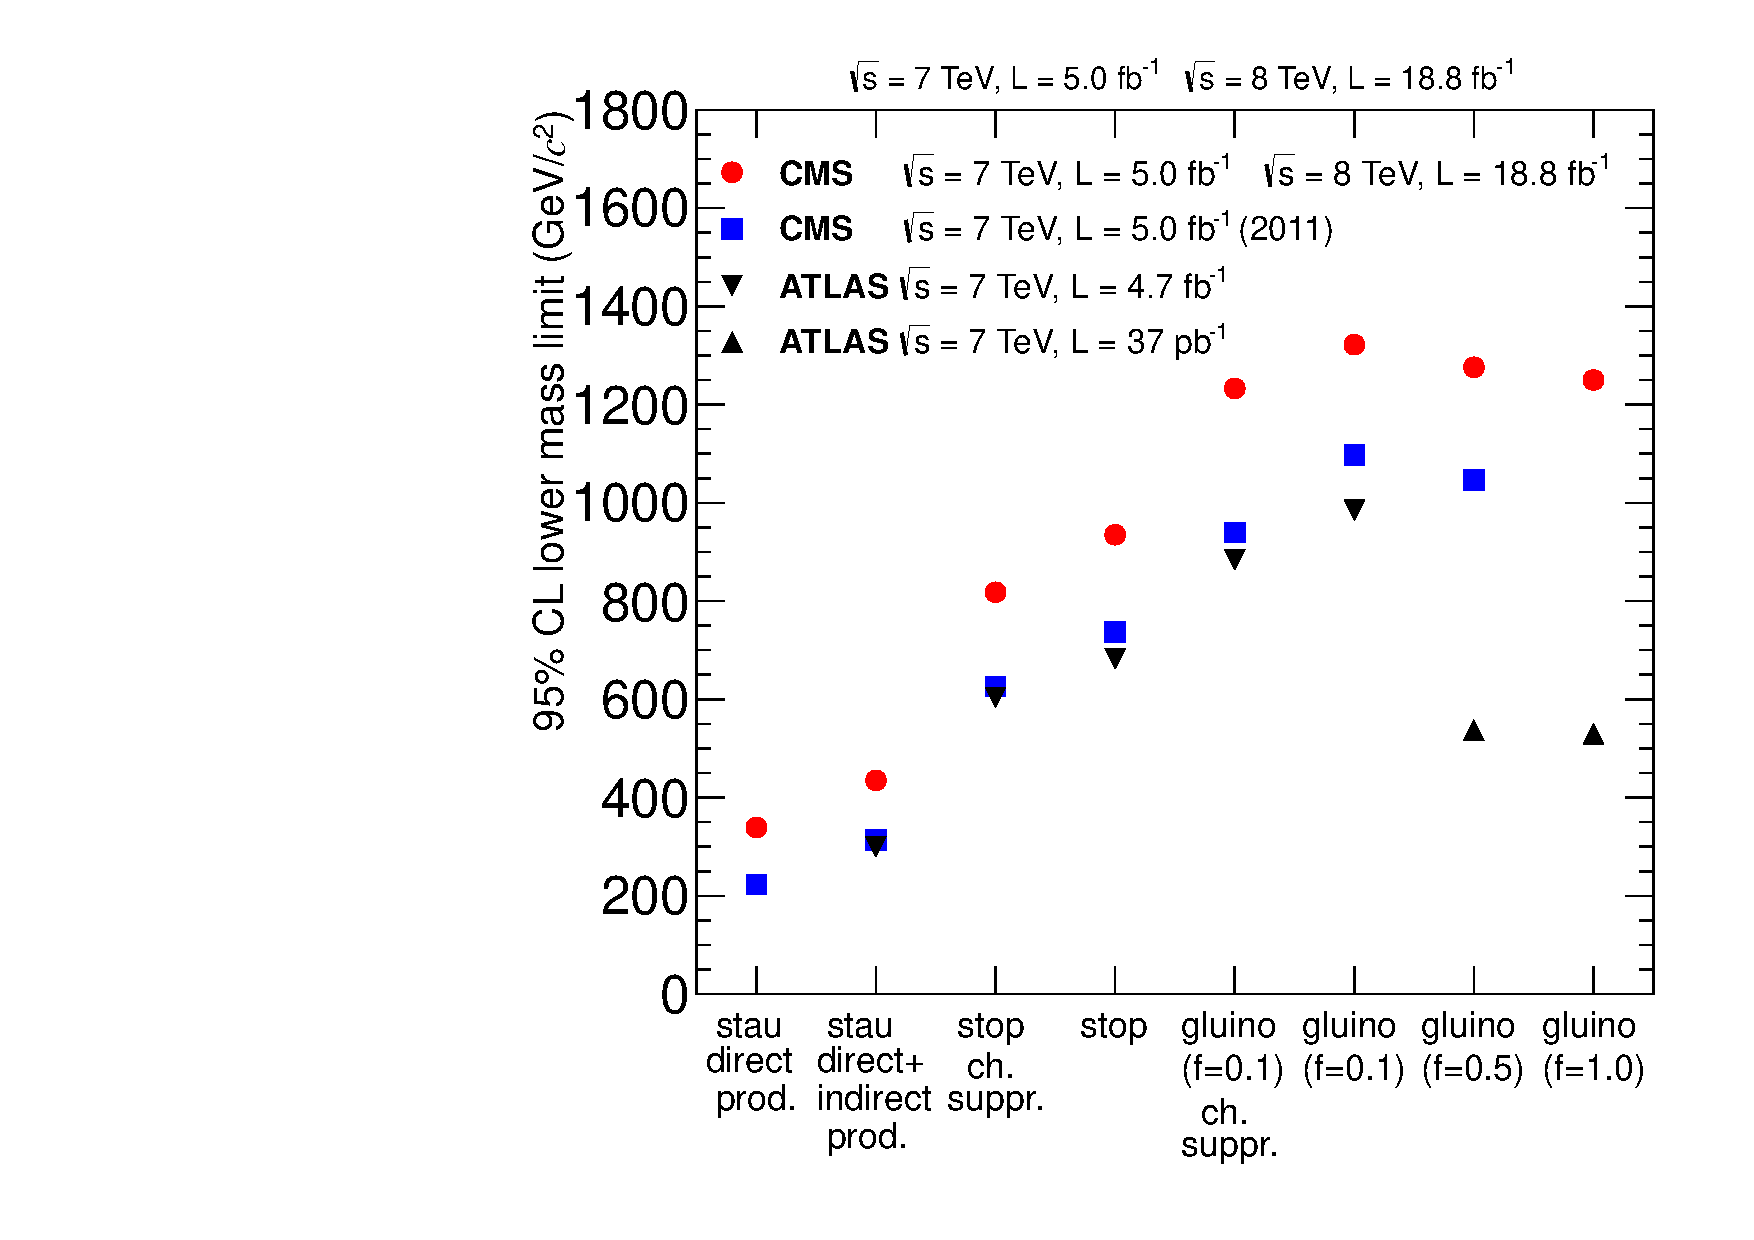
\includegraphics[clip=false, trim=0.0cm 0cm 0.0cm 0cm, width=0.68\textwidth]{figures/hscp_resultsNov2012}
 \end{center}
 \caption[Lower mass limits on HSCP produced in various SUSY models compared with previously published results]
{Lower mass limits at 95\% CL on various SUSY models compared with previously published results
~\cite{Aad:2011hz, Aad:2011yf, Aad:2011mb,Aad:2012vd, ATLASmCHAMPs, Khachatryan:2011ts, Chatrchyan:2012sp}. 
The model type is defined by the x-axis. 
}
   \label{fig:SUSYmasslimits}
\end{figure}

\begin{figure}
 \begin{center}
 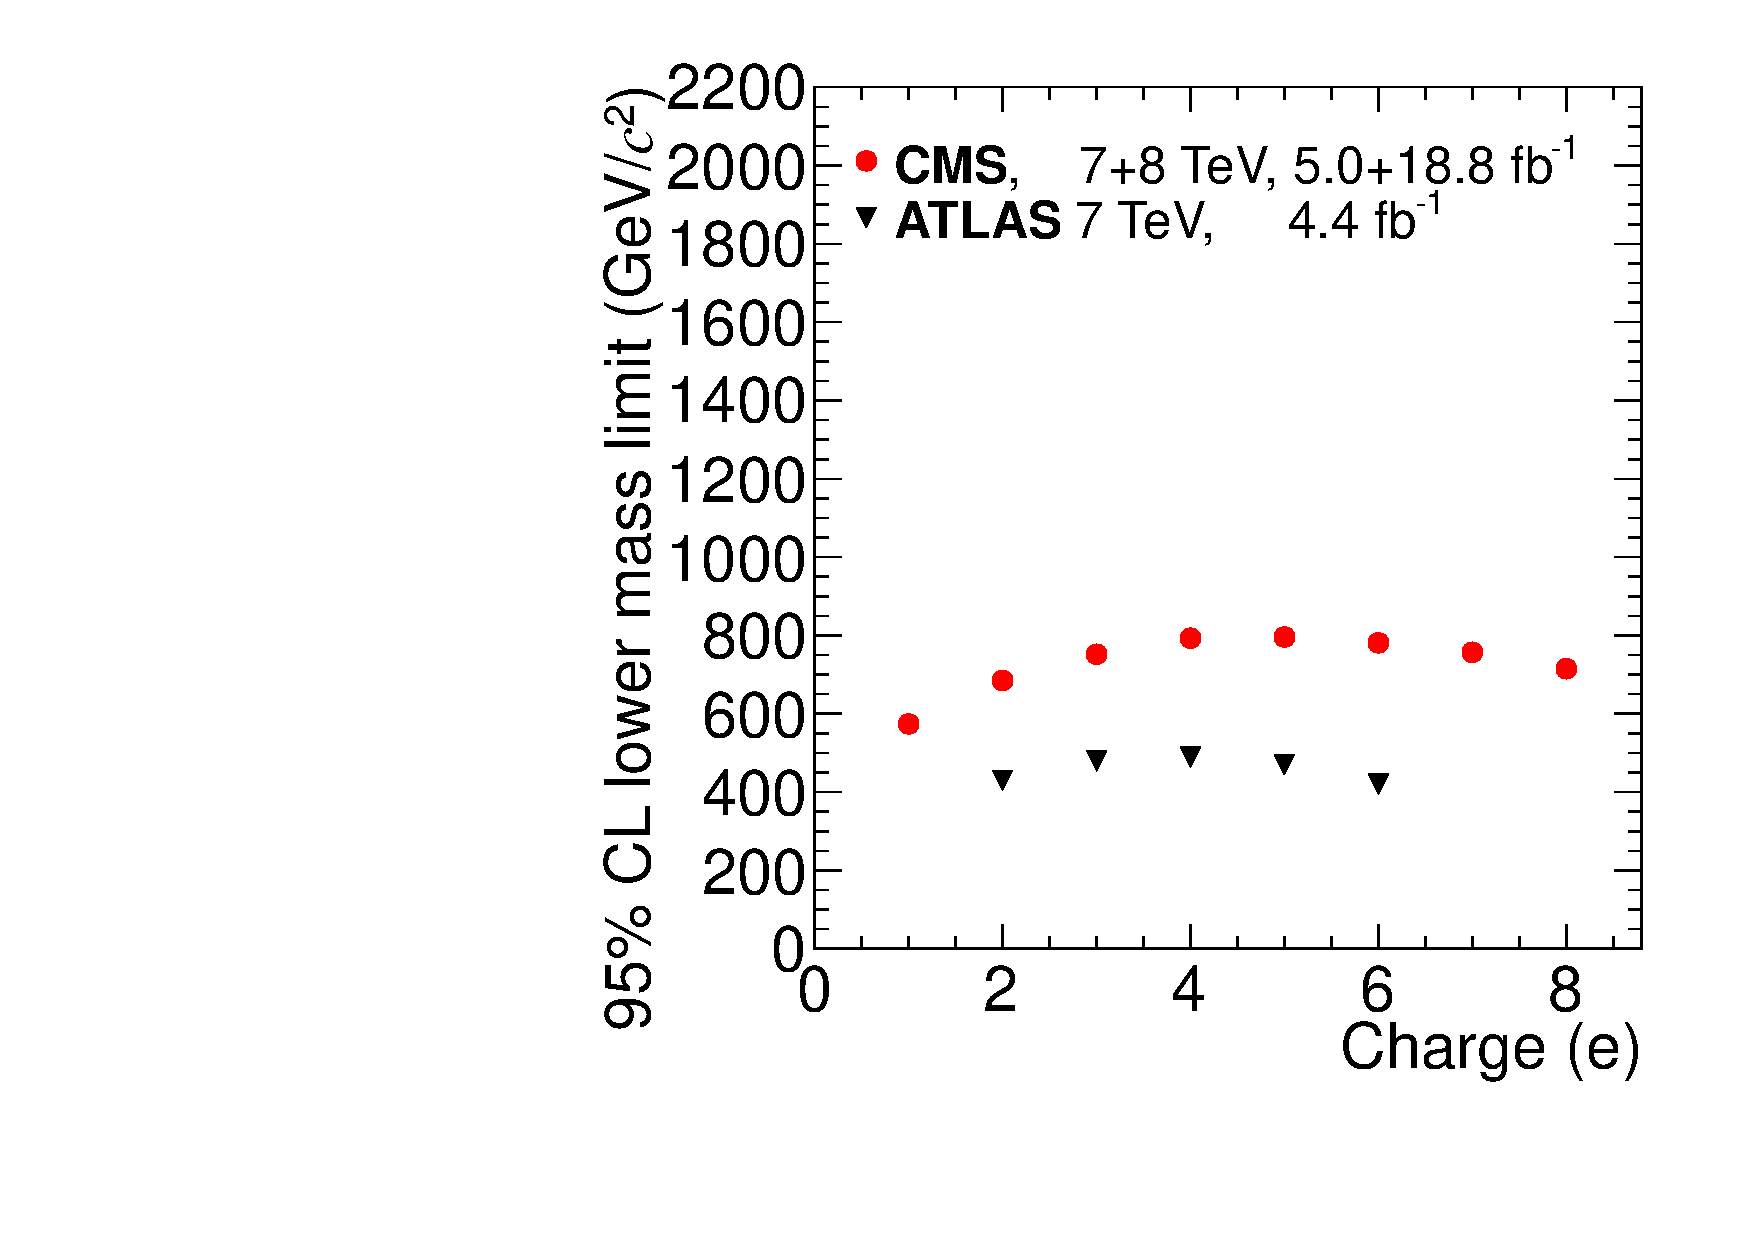
\includegraphics[clip=false, trim=0.0cm 0cm 0.0cm 0cm, width=0.68\textwidth]{figures/DYhscp_resultsNov2012}
 \end{center}
 \caption[Lower mass limits on HSCP produced with various charge compared with previously published results]
{Lower mass limits at 95\% CL for Drell--Yan like production of multiply charged particles versus electric charge compared with previously published results
~\cite{ATLASmCHAMPs}.
}
   \label{fig:HQmasslimits}
\end{figure}